\documentclass[a4paper]{book}
%\documentclass[a4paper]{ctexbook}
%\documentclass[a4paper]{ctexart}
\usepackage{ctex}
\usepackage{listings}
\usepackage{xcolor}
%\usepackage{xecolor}
\usepackage{graphicx}
\usepackage{geometry}
\usepackage{hyperref} %生成书签

%================================
% A.页面颜色
%================================
\definecolor{mypagecolor}{rgb}{0.78, 0.92, 0.8}
\pagecolor{mypagecolor}
\geometry{left=3.0cm, right=3.0cm, top=2.5cm, bottom=2.5cm}
%================================
% A.PDF标签
%================================
\hypersetup{
    colorlinks=true,
    bookmarksnumbered=true,
    pdftitle={My LaTeX2e note},
    pdfkeywords={LaTex, note},
}

\title{\Huge \bfseries 使用 \LaTeX 编写笔记}
\author{\huge 莫志烨}
\CTEXoptions[today=big]
\date{\Large \today}

%================================
% B.代码全局格式
%================================
\lstset{
    numbers=left,
    %numberstyle={\color{lightgray}},
    numberstyle={\color{green}},
    backgroundcolor={\color[RGB]{41, 47, 51}}, %背景颜色
    basicstyle={\color[RGB]{208, 214, 219}}, %普通字符串颜色
    stringstyle={\color[RGB]{0, 128, 0}}, %字符串颜色
    keywordstyle={\color[RGB]{101, 140, 230}}, %关键词颜色
    commentstyle={\color{gray}}, %注释颜色
    frame=none, %无边框
    breaklines=true, %自动分行
    language={[ANSI]C},
    captionpos=b,
}

%================================
% C.新命令定义
%================================
%\newcommand{OutputListing}[]{
%}

\begin{document}

%================================
% 1.标题
%================================
\chapter{标题}
\begin{titlepage}
\maketitle
\end{titlepage}

%================================
% 2.目录
%================================
\chapter{目录}
\tableofcontents

%================================
% 3.章节(每天日志入口)
%================================
\chapter{LaTex笔记}
\section{每天日志格式}

%1.每天日志格式

1.每天日志格式
\begin{lstlisting}[]
\chapter{2020年3月3日} //1.以日期为章节
\section{问题1} //2.以问题为小节!
\end{lstlisting}

2.插入代码格式1
\begin{lstlisting}[]
\begin{lstlistings}[caption={xxx}] %插入图注 //默认是C语法
\end{lstlistings}
\end{lstlisting}

2.插入代码格式2
\begin{lstlisting}[]
\lstinputlisting{lbuf.c}[caption={xxx}] %插入图注!
\end{lstlisting}

2.插入代码格式3
\begin{lstlisting}[]
\lstinline !code!
\end{lstlisting}

3.插入图片格式
\begin{lstlisting}[]
\graphicspath{{note_everyday/001_20200302/picture/}} %声明图片加载路径
\begin{figure}[h] %h:表示把图片放在当前位置
    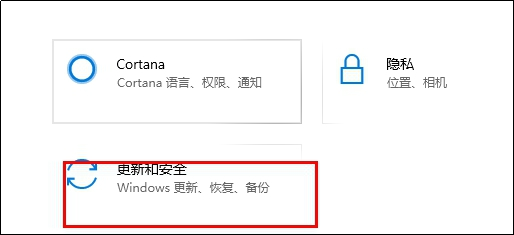
\includegraphics{001.jpg}
    \caption{第一步}
\end{figure}

\end{lstlisting}

\chapter{2020年3月2日 笔记}
\graphicspath{{note_everyday/001_20200302/picture/}}
\section{问题一:MMU学习}


1.步骤一:
\begin{figure}[h]
    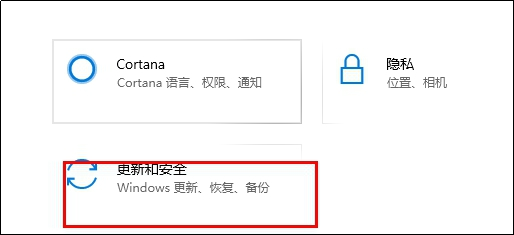
\includegraphics{001.jpg}
    \caption{第一步}
\end{figure}



\chapter{2020年3月5日 笔记}
\graphicspath{{note_everyday/004_20200305/picture/}}
\section{IIC协议}

1.接线 \\
    1)SCL: 时钟线, 由主机提供;\\
    2)SDA: 数据线;\\
    idle状态两个信号都会被拉高;\\

2.总线状态\\
    1)空闲状态: SCL和SDA都保持着高电平;\\
    2)start信号: 当SCL为高电平而SDA由高到低的跳变,表示产生一个起始条件;\\
    3)stop信号: 当SCL为高而SDA由低到高的跳变,表示产生一个停止条件;\\
    4)传输状态(忙): 处于start <---> stop之间;\\
        传输状态数据格式:数据采用: 8bit数据(发送方) + 1(接收方ack把SDA拉低);\\
        注: 整个过程取决于谁在控制SDA, 数据由发送方控制SDA状态发送, ack由接收方控制拉低(此时接收方为输入检测状态); \\

3.主机流程分析\\

4.主机流程分析\\


问题Q1:
1) 作为主机, 在发完数据后需要发stop信号时, 因为需要关enable, 但由于波特率太慢问题, 指令执行的太快, 在IIC模块还没发出stop信号, cpu就把模块关了;
\begin{lstlisting}[]
    if (end) {
    	iic_host_send_stop(iic_regs[id]); //stop singal
		//asm ("csync");
		delay(100);
		iic_disable(iic_regs[id]);
    }
\end{lstlisting}
    A.软件初步解决办法: 加delay();
    B.IC解决办法: 加stop pending, 等stop pending起来后再disable;

问题Q2: 作为主机, 在发完stop信号后, 再start, 信号会变得不正常(看stp看出时cnt问题);

\begin{figure}[h]
    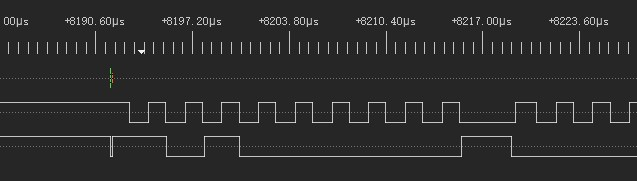
\includegraphics{q2_singal.jpg}
    \caption{第一步}
\end{figure}

问题Q3: 在读时不支持: 在不stop的情况下start
\begin{figure}[h]
    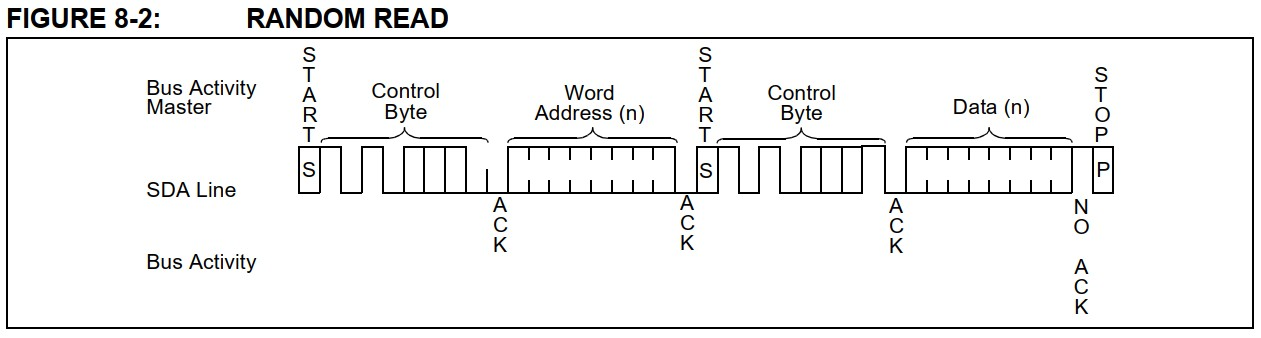
\includegraphics{eeprom_random_read.jpg}
    \caption{第一步}
\end{figure}




\chapter{2020年3月6日 笔记}
\graphicspath{{note_everyday/005_20200306/picture/}}
\section{VOA}

%Big companies are trying to keep their employees healthy by banning business trips. The decision, however, has been a hard blow to the travel industry, which has already been suffering because of the effects of the new coronavirus.
大型企业正试图通过禁止商务旅行来确保员工的健康。但是这一决定给已经因为新型冠状病毒遭受重创的旅游业造成了沉重打击。
Amazon, the American-based online business, has told its nearly 800,000 workers to postpone any unnecessary travel within the United States or around the world.
总部位于美国的网络公司亚马逊已经通知其近80万员工推迟在美国国内或全球范围内任何非必要的旅行。

Swiss food company Nestle told its 291,000 employees worldwide to limit local business travel and stop all international travel until March 15.
瑞士食品公司雀巢通知该公司在全球的29.1万名员工,在3月1日前要限制当地商务旅行并停止所有全球旅行。

France's L'Oréal, maker of beauty products, employs 86,000 people. It has announced a travel ban until March 31.
法国美容产品制造商欧莱雅公司雇用了8.6万名员工。该公司宣布3月31日前禁止旅行。

Major business gatherings, like the Mobile World Congress in Barcelona, have also been canceled.
诸如巴塞罗那世界移动大会之类的大型商业聚会也都被取消。

On Tuesday, Facebook confirmed it will not attend the South by Southwest conference in Austin, Texas. The event is supposed to start on March 13.
周二,脸书网确认将不会参加在德克萨斯州奥斯汀市举行的西南偏南大会。该活动原定于3月13日开幕。

In addition, the International Monetary Fund and the World Bank have announced they will replace their spring meetings in Washington with an online event.
此外,国际货币基金组织和世界银行宣布将通过线上活动替代他们在华盛顿的春季会议。

Robin Ottaway is president of Brooklyn Brewery. He canceled a trip to Seoul and Tokyo last week. He has suspended all travel to Asia and canceled a planned trip this month to Copenhagen.
罗槟·奥特韦是布鲁克林啤酒厂的总裁。他上周取消了前往首尔和东京的旅行。他已经暂停前往亚洲,并取消了本月原计划前往哥本哈根的旅行。

"I wasn't worried about getting sick. I'm a healthy 46-year-old man," Ottaway said. "My only worry was getting stuck in Asia or quarantined after returning to the U.S. And I'd hate to be a spreader of the virus."
奥特韦表示:“我不是害怕感染。我是一位46岁的健康男性。我唯一担心是被困在亚洲,或是回到美国后被隔离。我不想成为这种病毒的传播者。”

Effect on business travel
对商务旅行的影响

The cancellations and travel restrictions are hurting the travel industry. Business travel makes up around 26 percent of the total travel spending, or around $1.5 trillion per year, notes the Global Business Travel Association.
取消和旅行限制伤害了旅游业。全球商务旅行协会指出,商务旅行约占整个旅行支出的26%,即每年大约1.5万亿美元。

The association estimates the virus is costing the business travel industry $47 billion per month.
该协会估计该病毒每个月给商务旅行行业造成470亿美元的损失。

"It's a big deal," said Henry Harteveldt, a travel industry expert. He estimates that airline companies get 55 percent of their money from business travelers because they often sit in pricier business or first-class seats.
旅游行业专家亨特·哈特威尔特表示:“这是个大事件。”他估计航空公司55%对收入来自于商务旅客,因为他们通常乘坐价格更高的商务舱或头等舱。

Numbers from the Airlines Reporting Corporation show that airline ticket sales fell about 9 percent in late February, compared with a year earlier.
航空报告公司的数据显示,与去年同期相比,2月下旬的机票销售下降了大约9%。

Hotel operators are also worried about decreases in business travel. In the United States, hotels are expected to earn $46 billion from business travel this year, said the travel research service Phocuswright. No one believes that is possible now.
酒店经营者也在担心商务旅行的减少。旅游研究公司Phocuswright表示,美国酒店今年预计从商务旅行中赚到460亿美元。现在没人相信这能实现。

In the week through February 22, hotel occupancy rates in San Francisco were down 11 percent, noted STR, a company that researches hotel usage. Several major companies pulled out of the city's cybersecurity conference, which began in February.
研究酒店入住率的STR公司指出,截至2月22日的这个星期,旧金山酒店入住率下降了11%。几家重要公司退出了该市2月份开始举行的网络安全会议。

Some observers say it is wise for companies to postpone or cancel travel before things get worse. Worldwide, the coronavirus has sickened over 90,000 people. More than 3,000 have died from COVID-19, the disease resulting from the virus.
一些观察人士表示,企业在情况恶化前取消或推迟旅行是非常明智的。在全球范围内,这种冠状病毒已经导致9万人感染。超过3千人因为这种病毒引起的新型冠状病毒肺炎死亡。

Kevin Mitchell is chairman of the Business Travel Coalition. He is an expert in the ways large companies and governments can control travel costs. He notes that if a company puts an employee at risk, "you can be held responsible for their injury or death."
凯文·米切尔是商务旅行联盟的主席。他是大型企业和政府差旅成本控制方面的专家。他指出,如果企业将员工置于危险之中,“可能需要对他们的伤亡负责。”
By Susan Shand
05 March 2020
Big companies are trying to keep their employees healthy by banning business trips. The decision, however, has been a hard blow to the travel industry, which has already been suffering because of the effects of the new coronavirus.

Amazon, the American-based online business, has told its nearly 800,000 workers to postpone any unnecessary travel within the United States or around the world.

Swiss food company Nestle told its 291,000 employees worldwide to limit local business travel and stop all international travel until March 15.

Workers wearing protective gear spray disinfectant as a precaution against the coronavirus outbreak, in the departure terminal at the Rafik Hariri International Airport, in Beirut, Lebanon, Thursday, March 5, 2020.
France's L'Oréal, maker of beauty products, employs 86,000 people. It has announced a travel ban until March 31.

Major business gatherings, like the Mobile World Congress in Barcelona, have also been canceled.

On Tuesday, Facebook confirmed it will not attend the South by Southwest conference in Austin, Texas. The event is supposed to start on March 13.

In addition, the International Monetary Fund and the World Bank have announced they will replace their spring meetings in Washington with an online event.

Robin Ottaway is president of Brooklyn Brewery. He canceled a trip to Seoul and Tokyo last week. He has suspended all travel to Asia and canceled a planned trip this month to Copenhagen.

"I wasn't worried about getting sick. I'm a healthy 46-year-old man," Ottaway said. "My only worry was getting stuck in Asia or quarantined after returning to the U.S. And I'd hate to be a spreader of the virus."

Effect on business travel

The cancellations and travel restrictions are hurting the travel industry. Business travel makes up around 26 percent of the total travel spending, or around 1.5 trillion per year, notes the Global Business Travel Association.

The association estimates the virus is costing the business travel industry 47 billion per month.

"It's a big deal," said Henry Harteveldt, a travel industry expert. He estimates that airline companies get 55 percent of their money from business travelers because they often sit in pricier business or first-class seats.

Numbers from the Airlines Reporting Corporation show that airline ticket sales fell about 9 percent in late February, compared with a year earlier.

Hotel operators are also worried about decreases in business travel. In the United States, hotels are expected to earn 46 billion from business travel this year, said the travel research service Phocuswright. No one believes that is possible now.

In the week through February 22, hotel occupancy rates in San Francisco were down 11 percent, noted STR, a company that researches hotel usage. Several major companies pulled out of the city's cybersecurity conference, which began in February.

Some observers say it is wise for companies to postpone or cancel travel before things get worse. Worldwide, the coronavirus has sickened over 90,000 people. More than 3,000 have died from COVID-19, the disease resulting from the virus.

Kevin Mitchell is chairman of the Business Travel Coalition. He is an expert in the ways large companies and governments can control travel costs. He notes that if a company puts an employee at risk, "you can be held responsible for their injury or death."

I'm Susan Shand.

The Associated Press reported this story. Susan Shand adapted it for VOA Learning English. George Grow was the editor.

Write to us in the Comments Section or on 51VOA.COM.

%________________________________________________________________

Words in This Story
outbreak – n. a sudden start or increase of fighting or disease

cosmetics – n. a substance (such as a cream, lotion, or powder) that you put on your face or body to improve your appearanc

standstill – n. a state in which all activity or motion is stopped

quarantine – v. to keep (a person or animal) away from others to prevent a disease from spreading

cybersecurity – n. ways to keep internet data away from criminals


\chapter{2020年3月16日 笔记}
\graphicspath{{note_everyday/001_20200316/picture/}}
\section{VOA}
%\begin{document}
\begin{lstlisting}[]
By Susan Shand
15 March 2020
Billionaire art collector David Nahmad cannot remember why he bought "Nature Morte," a small oil painting by Pablo Picasso.
Nahmad owns about 300 of Picasso's works. So, his forgetfulness is understandable.
"We bought so many Picassos now, I don't remember the... reason," Nahmad said to Associated Press reporters from his home in Monaco.
The 72-year-old started dealing art with his brothers in the 1960s, paying as little as 5,000 for pieces by Picasso and building the collection of works that made them into billionaires.
"Nature Morte" is the smallest painting Nahmad has. And it is about to belong to someone else. It will be sold to raise money for charity later this month.
Raffle tickets will be sold online and are 100 euros each. The winner of a similar Picasso raffle in 2013 was a 23-year-old worker from Pennsylvania.
Nahmad is one of the art world's most important art dealers. He will receive over 1 million for "Nature Morte." But he said the piece is worth "at least two, three times" that.
"This raffle would not have succeeded if the name was not Picasso. I tried to propose other artists' names. But it would not work, because they wanted a name that would appeal to everybody. It has to be Picasso. Picasso is the magic name," he said.
The value of Nahmad's collection is estimated to be about 3 billion. But he himself will not say what the exact value is.
"I don't think people care about the number of works, but about their quality," he said.
Nahmad said the possibility of giving up "Nature Morte" has made him look more closely at the small still life painting. It shows a newspaper and a glass of alcohol on a wood table.
"I think this painting is extremely chic," Nahmad said.
The raffle will be held in Paris on March 30. The organizers hope to sell 200,000 tickets. The money the event raises will help provide water for villagers in Cameroon, Madagascar and Morocco.
Nahmad believes that Picasso, who died in 1973, would have liked the raffling of his works to the public.
"Picasso was very generous," Nahmad said. "He wanted his art to be collected by all kinds of people, not only by the super-rich."
Nahmad's hope is that the winner of "Nature Morte" will be someone who loves the work. If not, "I will be very unhappy" and "would like to buy it back," Nahmad said.
"There's nothing worse than to own something without understanding that thing," he said.
I'm Susan Shand.
The Associated Press reported this story. Susan Shand adapted it for VOA Learning English. Ashley Thompson was the editor.
Write to us in the Comments Section or on 51VOA.COM.

\newline
%________________________________________________________________

Words in This Story
charity - n. the act of giving money, food, or other kinds of help to people who are poo

raffle – n. a contest that a group or organization uses to earn money and that involves people buying numbered tickets in exchange for a chance to win a prize

propose – v. to suggest (something, such as a plan or theory) to a person or group of people to consider

magic - n. special power, influence, or skill

chic – adj. following the current fashion or style : fashionable and appealing

generous - adj. freely giving or sharing money and other valuable things

%\end{document}
\end{lstlisting}





\chapter{2020年3月18日 笔记}
\graphicspath{{note_everyday/001_20200318/picture/}}
\section{VOA}
By Susan Shand
16 March 2020
U.S. researchers on Monday gave the first shot to the first volunteer in a test for an experimental coronavirus vaccine. Scientists at the Kaiser Permanente Washington Health Research Institute in Seattle are carrying out the trial.

"We're team coronavirus now," Kaiser Permanente scientist Dr. Lisa Jackson said.

The Associated Press watched the first volunteer, an employee of a small technology company, receive the injection. In total, the trial study will give 45 young, healthy volunteers two doses of the vaccine, one month apart.

Public health officials say it will take 12 to 18 months for a vaccine to be approved.

The vaccine being tested in Seattle was developed by the U.S. National Institutes of Health and the biotechnology company Moderna. There is no chance the volunteers will get sickened from the vaccine; it does not contain the virus.

The goal of the trial is only to make sure the vaccine does not have any worrisome side effects. Once it is proven to be safe, larger trials will begin.

Research groups around the world are working to create a vaccine for COVID-19, the disease caused by the new coronavirus. They are creating different kinds of vaccines. Some are shots developed from new technologies. These are faster to produce than traditional shots and may be stronger. Some research groups are even aiming for temporary vaccines, which would keep people safe for a month or two while longer-lasting protection is developed.

Next month, Inovio Pharmaceuticals will begin testing the safety of its vaccine in the American states of Pennsylvania and Missouri. Similar tests will then take place in China and South Korea.

Even if early tests go well, "you're talking about a year to a year and a half" before any vaccine could be ready for widespread use, said Dr. Anthony Fauci. He is director of the NIH's National Institute of Allergy and Infectious Diseases.

Vaccine manufacturers are required to do additional studies on thousands of people to be sure a vaccine does not cause harm. But waiting is hard for the fearful public.

U.S. President Donald Trump has been pushing for a vaccine. He recently said that the work is "moving along very quickly" and that he hoped to see a vaccine "soon."

There are no proven treatments for COVID-19. In China, scientists have been experimenting with HIV drugs as well as an experimental drug named remdesivir, which was created to fight Ebola.

In the United States, the University of Nebraska Medical Center also began testing remdesivir in some Americans who were found to have COVID-19.

For most people, the new coronavirus causes mild sickness, including a fever and cough. But for older people and people with serious health problems, it can cause more severe illness, including pneumonia.

The worldwide outbreak has sickened more than 175,000 people and left more 6,000 dead.

I'm Ashley Thompson.

The Associated Press reported this story. Susan Shand adapted it for Learning English. George Grow was the editor.\newline

\underline{uuuuuuuuuuuuuuuuuuuuuuuuuuuuuuu}

Words in This Story
clinical – adj. medical or scientific work done with human beings

dose – n. a prescribed amount of medication

pneumonia – n. a disease of the lungs that makes breathing difficult

outbreak – n. the sudden occurrence of war or disease


U.S. researchers on Monday gave the first shot to the first volunteer in a test for an experimental coronavirus vaccine. Scientists at the Kaiser Permanente Washington Health Research Institute in Seattle are carrying out the trial.
周一,美国研究人员对参与试验性冠状病毒疫苗测试的第一位志愿者进行了注射。西雅图市凯撒华州卫生健康研究所的科学家们正在进行这项试验。
"We're team coronavirus now," Kaiser Permanente scientist Dr. Lisa Jackson said.
凯撒华州卫生健康研究所的科学家莉莎·杰克逊表示:“我们现在开始驯服冠状病毒。”

The Associated Press watched the first volunteer, an employee of a small technology company, receive the injection. In total, the trial study will give 45 young, healthy volunteers two doses of the vaccine, one month apart.
美联社观察了首位志愿者接受疫苗注射的过程,这位志愿者是一家小型技术公司的雇员。这项试验性研究将为共计45位健康的年轻志愿者注射两剂疫苗,注射间隔为一个月。

Public health officials say it will take 12 to 18 months for a vaccine to be approved.
公共卫生官员表示,疫苗获批需要12到18个月时间。

The vaccine being tested in Seattle was developed by the U.S. National Institutes of Health and the biotechnology company Moderna. There is no chance the volunteers will get sickened from the vaccine; it does not contain the virus.
西雅图测试的这种疫苗是由美国国立卫生研究院和Moderna生物技术公司所研制。志愿者不会被疫苗感染,疫苗并不包含病毒。

The goal of the trial is only to make sure the vaccine does not have any worrisome side effects. Once it is proven to be safe, larger trials will begin.
这次试验的目的只是为了确保疫苗没有任何令人担忧的副作用。一旦安全性得到验证,就将会进行更大规模的试验。

Research groups around the world are working to create a vaccine for COVID-19, the disease caused by the new coronavirus. They are creating different kinds of vaccines. Some are shots developed from new technologies. These are faster to produce than traditional shots and may be stronger. Some research groups are even aiming for temporary vaccines, which would keep people safe for a month or two while longer-lasting protection is developed.
世界各地的研究小组都在努力开发针对新冠肺炎的疫苗。他们正在开发不同类型的疫苗。有些是采用新技术开发的针剂。与传统针剂相比,它们的生产速度更快,并且可能更强。一些研究小组甚至计划开发临时性疫苗,它将在长效疫苗开发期间给人们提供一到两个月的保护。

Next month, Inovio Pharmaceuticals will begin testing the safety of its vaccine in the American states of Pennsylvania and Missouri. Similar tests will then take place in China and South Korea.
下个月,诺维欧制药将会开始在美国宾夕法尼亚州和密苏里州测试其疫苗的安全性。随后中国和韩国也将进行类似的测试。

Even if early tests go well, "you're talking about a year to a year and a half" before any vaccine could be ready for widespread use, said Dr. Anthony Fauci. He is director of the NIH's National Institute of Allergy and Infectious Diseases.
安东尼·福西博士表示,即使早期测试进展顺利,任何疫苗广泛投入使用之前也需要一年到一年半时间。福西是美国国立卫生研究院国家过敏和传染病研究所所长。

Vaccine manufacturers are required to do additional studies on thousands of people to be sure a vaccine does not cause harm. But waiting is hard for the fearful public.
疫苗生产商必须对数千人进行进一步研究,以确保疫苗不会造成伤害。但是等待对恐慌民众来说是很艰难的。

U.S. President Donald Trump has been pushing for a vaccine. He recently said that the work is "moving along very quickly" and that he hoped to see a vaccine "soon."
美国总统川普一直在推动疫苗问世。他最近表示,这项工作进展很快,他希望很快看到疫苗问世。

There are no proven treatments for COVID-19. In China, scientists have been experimenting with HIV drugs as well as an experimental drug named remdesivir, which was created to fight Ebola.
目前针对新冠肺炎并没有被证实有效的疗法。在中国,科学家们一直在试验艾滋病药物,以及一种名为瑞德西韦、开发用于抗击埃博拉的试验性药物。

In the United States, the University of Nebraska Medical Center also began testing remdesivir in some Americans who were found to have COVID-19.
在美国,内布拉斯加大学医学中心也开始在一些感染新冠肺炎的美国患者身上测试瑞德西韦。

For most people, the new coronavirus causes mild sickness, including a fever and cough. But for older people and people with serious health problems, it can cause more severe illness, including pneumonia.
对大多数人来说,新冠病毒会引起包括发烧和咳嗽在内的轻度疾病。但是对老年人和本身患有严重疾病的人群来说,它会导致包括肺炎在内的更严重的疾病。

The worldwide outbreak has sickened more than 175,000 people and left more 6,000 dead.
新冠疫情全球爆发已经导致17.5万人感染,并造成6千多人死亡。

I'm Ashley Thompson.
我是阿什利·汤普森。(51VOA.COM原创翻译,禁止转载,违者必究!)




\chapter{2020年3月23日 笔记}
\graphicspath{{note_everyday/001_20200323/picture/}}
\section{VOA}
\href{https://www.51voa.com/VOA_Special_English/when-the-cat-s-away-the-mice-will-play-84151.html}{文章链接}
By Anna Matteo
21 March 2020
Now, it's time for Words and Their Stories, a program from VOA Learning English.
The internet has taught us many things. One important lesson is this: Cats are funny, strange and often unpredictable animals. Their quirky personalities have made cats popular as household pets in homes across the United States.
And they are great hunters. Mice are often on their top five kill list. But sometimes, a cat will not kill the animal it catches. Instead, the catch becomes kind of a toy or plaything.
The cat seizes a mouse. Then lets it go. Catches it. Lets it go. Over and over again! It is good fun for the cat but frightening for the poor mouse.
So, if you play cat and mouse with someone, you play a power game with them. You, the person with the power, are the cat. Maybe you pretend to give the other person something they want but then take it away. You toy with them. We often call a situation like this a cat-and-mouse game. For example, a child might offer something sweet to her little brother and then take it away when he reaches for it.
A cat-and-mouse game is filled with lots of action: chases, near captures and repeated escapes. In extreme cases, a cat-and-mouse game is never-ending.
Now, let's leave the game of cat and mouse and talk about playing in a different way.
Let's imagine a classroom filled with young children. The teacher must leave the room for a couple of minutes. At first, everyone is well-behaved. But the longer the teacher is gone, the more the class acts up. It starts out slowly. Someone throws a piece of paper. A couple of students get up and walk around. Others start laughing loudly. Someone yells! Suddenly, all of the students are doing things they would never do with the teacher in the room.
But you know what we say: When the cat's away, the mice will play!
This expression means that people sometimes misbehave when no one is there to watch them. So, the teacher is the cat and the students are the mice.
We often use this expression when talking about children and parents, employees and office supervisors and even people in committed relationships.
And that brings us to the end of this Words and Their Stories.
Until next time ... I'm Anna Matteo.
Anna Matteo wrote this story for VOA Learning English. George Grow was the editor.

\underline{-------------------------------------}

Words in This Story
lesson – n. an activity that you do in order to learn something

quirky – adj. unusual in especially an interesting or appealing way

pet – n. a tame animal kept as a companion rather than for work

pretend – v. to give a false appearance of being, possessing, or performing





Now, it's time for Words and Their Stories, a program from VOA Learning English.
现在是美国之音慢速英语词汇掌故节目时间。
The internet has taught us many things. One important lesson is this: Cats are funny, strange and often unpredictable animals. Their quirky personalities have made cats popular as household pets in homes across the United States.
互联网教会了我们很多东西。其中一个重要教训就是:猫是一种有趣、奇怪而且往往不可捉摸的动物。这种古怪个性使得猫成为了全美国最受欢迎的家庭宠物。

And they are great hunters. Mice are often on their top five kill list. But sometimes, a cat will not kill the animal it catches. Instead, the catch becomes kind of a toy or plaything.
同时它们是伟大的捕手。老鼠通常是它们消灭名单的前五位。但是有时候猫不会吃掉它们抓到的动物。相反,猎物会变成它们的玩物。

The cat seizes a mouse. Then lets it go. Catches it. Lets it go. Over and over again! It is good fun for the cat but frightening for the poor mouse.
猫抓住老鼠,然后放掉,再抓住,再放掉,就这样一遍遍重复。对猫来说这很好玩,对可怜的老鼠来说却是恐惧。

So, if you play cat and mouse with someone, you play a power game with them. You, the person with the power, are the cat. Maybe you pretend to give the other person something they want but then take it away. You toy with them. We often call a situation like this a cat-and-mouse game. For example, a child might offer something sweet to her little brother and then take it away when he reaches for it.
因此,如果你和某人玩猫鼠游戏,意思是你跟他们玩权力游戏。你作为有权势的一方,就是猫。可能你会假装给某人他们想要的东西,然后又将其拿走。你在玩弄他们。我们通常称这种情况是猫鼠游戏。例如,某个孩子可能会给她弟弟一些甜食,然后在弟弟伸手要够时又把它拿走。

A cat-and-mouse game is filled with lots of action: chases, near captures and repeated escapes. In extreme cases, a cat-and-mouse game is never-ending.
猫鼠游戏有很多动作:追逐、近距离捕获以及反复逃跑。在某些极端情况下,猫鼠游戏永远没有结束的时候。

Now, let's leave the game of cat and mouse and talk about playing in a different way.
现在让我们放下猫鼠游戏,谈谈另一种玩法。

Let's imagine a classroom filled with young children. The teacher must leave the room for a couple of minutes. At first, everyone is well-behaved. But the longer the teacher is gone, the more the class acts up. It starts out slowly. Someone throws a piece of paper. A couple of students get up and walk around. Others start laughing loudly. Someone yells! Suddenly, all of the students are doing things they would never do with the teacher in the room.
我们假设一个教室里坐满了小孩子。老师必须离开教室几分钟时间。起初每个人都表现得很棒。但是老师离开的时间越长,班上捣蛋的就越多。它是慢慢开始的。有人扔了一张纸,几个学生站起来到处走。其他人开始大声说笑。有人大喊。突然,所有学生都在做老师在教室时他们永远不会去做的事情。

But you know what we say: When the cat's away, the mice will play!
但是你知道我们说的:猫儿不在,老鼠成精。

This expression means that people sometimes misbehave when no one is there to watch them. So, the teacher is the cat and the students are the mice.
这句表达的意思是有时候人们在没管的时候会乱来。所以,老师就是猫,学生们是老鼠。

We often use this expression when talking about children and parents, employees and office supervisors and even people in committed relationships.
我们在谈论孩子和父母,员工和领导,以及存在固定关系的人们时常常会用到这句表达。

And that brings us to the end of this Words and Their Stories.
以上就是本期词汇掌故节目的全部内容。

Until next time ... I'm Anna Matteo.
我们下次节目再会。我是安娜·马特奥。

(51VOA.COM原创翻译,禁止转载,违者必究!)






\chapter{2020年3月24日 笔记}
\graphicspath{{note_everyday/001_20200324/picture/}}
\section{VOA}
\href{https://www.51voa.com/VOA_Special_English/can-the-world-copy-south-korea-s-coronavirus-plan-84162.html}{Can the World Copy South Korea’s Coronavirus Plan?} \newline

By Susan Shand
23 March 2020
On Thursday morning, VOA's reporter in Seoul, William Gallo, received a text message from South Korea's emergency alert system. The message appeared on his telephone. He has received such texts hundreds of times during the coronavirus outbreak.

Someone in Gallo's Seoul neighborhood — a 35-year-old man — had tested positive for the virus. The text message provided a link to a government website that listed everything about the man's activities for the past two days.

The man apparently arrived at Seoul's Incheon airport at about nine in the morning. He took a train to a train station near Gallo's home, and then went to a small food store. Five hours later, he went to a restaurant. More information followed.

By now, messages like this one are commonplace in South Korea. Gallo says his phone receives more than 10 messages about infections in his neighborhood on some days. When he goes to other parts of Seoul, his phone provides information about cases in those neighborhoods.

To prepare these messages, South Korea uses in-person interviews. It also uses large amounts of personal information, bank records, phone information as well as video from cameras around the city.

This is possible because South Korean lawmakers changed privacy laws after the outbreak of Middle East Respiratory Syndrome (MERS) in 2015. The disease caused 39 deaths in the country. Now, during dangerous outbreaks, officials can easily get everyone's private information without a court order.

The plan has worked

As a result, South Korea has been able to identify areas with more than one coronavirus case and quickly investigate the path of the infection. It can tell those infected to stay home and warn the public to avoid that area.

The result has been stunning. South Korea has reported one of the lowest coronavirus death rates in the world: as of Monday, only 111 people have died out of 8,961 cases.

The rate of new infections has also decreased. After reaching 909 new cases a day on February 29, South Korea reported just 64 new cases on Monday.

South Korea's methods of fighting coronavirus have been praised as the model of how to contain the virus. It avoids forced restrictions on movement and does not lead to widespread closure of businesses.

Some people, however, are worried about the loss of privacy.

Kenneth Roth is executive director of Human Rights Watch. He told VOA his organization is worried governments may use the threat of coronavirus to increase their powers of surveillance.

"Once we allow them to be regularly used and give up... our right of privacy, it will be very difficult" to end it, said Roth.

If South Korea is reducing privacy in exchange for fighting the virus, many South Koreans seem to accept it happily.

Amid the coronavirus crisis, South Korean President Moon Jae-in is enjoying his highest approval ratings in months.

In some ways, South Korea's government is helped in the fight against coronavirus by what remains of its authoritarian past, says Lee Sang-sin. He is an expert on political science and public opinion at the Korean Institute for National Unification.

South Korea has a national registration system, he noted. Everyone has an identification number that must be given when buying a telephone. That has made it easier for government officials to find suspected coronavirus patients.

There are other reasons it may be difficult for countries to use the South Korean system to fight coronavirus.

South Korea is a small country, and is home to 51 million people. More than 50 percent live in cities and are easy to find.

Most importantly, everyone in South Korea, including non-citizens, is part of a national healthcare system.

Within the system, South Korea quickly built about 50 drive-thru testing centers. These have been praised internationally for their safety and effectiveness.

Back to normal?

As the number of new coronavirus infections decreases, life in Seoul has begun to return to the way it was before the outbreak.

Schools are still closed, but people are out in public spaces and open areas.

I'm Ashley Thompson.

VOA's William Gallo reported this story. Susan Shand adapted it for Learning English. George Grow was the editor.

\underline{-------------------------------------------------------------------}

Words in This Story
outbreak - n. the sudden appearance of a sickness
positive - adj. a good outcome
stunning - adj. an extraordinary event
surveillance - n. following and watching a person
allow - v. to let someone do something
authoritarian - adj. oppressive, lacking democracy \newline






\href{https://files.21voa.com/202003/can-the-world-copy-south-korea-s-coronavirus-plan.mp3}{Can the World Copy South Korea’s Coronavirus Plan? Record} \newline

\\\href{https://www.51voa.com/VOA_Special_English/can-the-world-copy-south-korea-s-coronavirus-plan-84162_1.html}{Can the World Copy South Korea’s Coronavirus Plan? Translate} \newline

On Thursday morning, VOA's reporter in Seoul, William Gallo, received a text message from South Korea's emergency alert system. The message appeared on his telephone. He has received such texts hundreds of times during the coronavirus outbreak.
周四早上,美国之音驻首尔记者威廉·加洛收到了韩国紧急警报系统发来的一条短信。这条短信发到了他的手机上。在冠状病毒爆发期间,他已经收到了数百条此类短信。
Someone in Gallo's Seoul neighborhood — a 35-year-old man — had tested positive for the virus. The text message provided a link to a government website that listed everything about the man's activities for the past two days.
加洛在首尔的邻居中有一位35岁男子新冠病毒检测结果呈阳性。这条短信提供了一条指向政府网站的链接,该网站列出了该男子过去两天的所有活动信息。

The man apparently arrived at Seoul's Incheon airport at about nine in the morning. He took a train to a train station near Gallo's home, and then went to a small food store. Five hours later, he went to a restaurant. More information followed.
该男子显然是在早上约九点抵达首尔仁川机场。他坐地铁去了加洛家附近的地铁站,然后去了一家小食品店。5个小时后,他去了一家餐馆。后面还有更多信息。

By now, messages like this one are commonplace in South Korea. Gallo says his phone receives more than 10 messages about infections in his neighborhood on some days. When he goes to other parts of Seoul, his phone provides information about cases in those neighborhoods.
如今类似的短信在韩国很普遍。加洛表示,他的手机每天都收到10多条关于附近街区这几天感染病例的短信。当他去首尔其它地方时,他的手机会提供这些街区感染病例的信息。

To prepare these messages, South Korea uses in-person interviews. It also uses large amounts of personal information, bank records, phone information as well as video from cameras around the city.
为了准备这些短信,韩国采取了面谈方式。它还使用大量个人信息、银行记录、电话信息以及整个城市的摄像机拍摄的视频。

This is possible because South Korean lawmakers changed privacy laws after the outbreak of Middle East Respiratory Syndrome (MERS) in 2015. The disease caused 39 deaths in the country. Now, during dangerous outbreaks, officials can easily get everyone's private information without a court order.
这在韩国是可能实现的,因为韩国议员在2015年中东呼吸综合征爆发后修改了隐私法。这种疾病在该国导致了39人死亡。现在,在爆发危险的情况下,有关官员无需法院命令就能轻松获取每个人的隐私信息。

The plan has worked
方案奏效

As a result, South Korea has been able to identify areas with more than one coronavirus case and quickly investigate the path of the infection. It can tell those infected to stay home and warn the public to avoid that area.
结果,韩国得以确定有多起冠状病毒病例的区域,并迅速调查感染途径。它可以告诉感染者留在家里,并警告公众避开该区域。

The result has been stunning. South Korea has reported one of the lowest coronavirus death rates in the world: as of Monday, only 111 people have died out of 8,961 cases.
结果令人震惊。韩国是全球冠状病毒死亡率最低的国家之一:截至周一,该国8961起病例中只有111人死亡。

The rate of new infections has also decreased. After reaching 909 new cases a day on February 29, South Korea reported just 64 new cases on Monday.
新增感染率也有所下降。在2月29日达到一天新增909例确诊病例之后,韩国在周一仅报告了64起新病例。

South Korea's methods of fighting coronavirus have been praised as the model of how to contain the virus. It avoids forced restrictions on movement and does not lead to widespread closure of businesses.
韩国抗击冠状病毒的方法已经被誉为遏制该病毒的典范。它避免了对行动的强制性限制,并且不会导致商业大范围关闭。

Some people, however, are worried about the loss of privacy.
然而有人担心丢掉隐私。

Kenneth Roth is executive director of Human Rights Watch. He told VOA his organization is worried governments may use the threat of coronavirus to increase their powers of surveillance.
肯尼斯·罗斯是人权观察组织的执行董事。他对美国之音表示,该组织担心政府可能会利用冠状病毒的威胁来增强其监视能力。

"Once we allow them to be regularly used and give up... our right of privacy, it will be very difficult" to end it, said Roth.
罗斯表示:“一旦我们允许个人信息被定期使用,并且放弃我们的隐私权,要阻止它可就非常难了。”

If South Korea is reducing privacy in exchange for fighting the virus, many South Koreans seem to accept it happily.
如果韩国通过减少隐私权来换取抗击病毒,很多韩国人似乎很乐意接受。

Amid the coronavirus crisis, South Korean President Moon Jae-in is enjoying his highest approval ratings in months.
在冠状病毒危机中,韩国总统文在寅享有数月来的最高支持率。

In some ways, South Korea's government is helped in the fight against coronavirus by what remains of its authoritarian past, says Lee Sang-sin. He is an expert on political science and public opinion at the Korean Institute for National Unification.
李尚允表示,从某种意义上说,韩国政府的独裁历史为抗击冠状病毒提供了帮助。他是大韩民国统一研究所的政治学和舆论专家。

South Korea has a national registration system, he noted. Everyone has an identification number that must be given when buying a telephone. That has made it easier for government officials to find suspected coronavirus patients.
他指出,韩国有国家登记系统。每个人都有身份证号码,在购买电话时必须提供该号码。这让政府更容易找出冠状病毒疑似患者。

There are other reasons it may be difficult for countries to use the South Korean system to fight coronavirus.
还有其它原因让各国可能难以采用韩国抗击冠状病毒的体系。

South Korea is a small country, and is home to 51 million people. More than 50 percent live in cities and are easy to find.
韩国是一个只有5100万人口的小国家。超过50\%的人口居住在城市中,可以轻易找出来。

Most importantly, everyone in South Korea, including non-citizens, is part of a national healthcare system.
更重要的是,韩国包括非公民在内的所有人都是国家医疗保健系统的一部分。

Within the system, South Korea quickly built about 50 drive-thru testing centers. These have been praised internationally for their safety and effectiveness.
在该系统下,韩国迅速建立了约50个“得来速”检测中心。其安全性和有效性得到了全球赞誉。

Back to normal?
回归正常?

As the number of new coronavirus infections decreases, life in Seoul has begun to return to the way it was before the outbreak.
随着冠状病毒新增感染数量的减少,首尔的生活已经开始恢复到疫情爆发前的状态。

Schools are still closed, but people are out in public spaces and open areas.
学校仍然关闭,但是人们都出门走进了公共场所和空旷区域。

I'm Ashley Thompson.
我是阿什利·汤普森。(51VOA.COM原创翻译,禁止转载,违者必究!) \newline






\chapter{2020年3月25日 笔记}
\graphicspath{{note_everyday/010_20200325/picture/}} %声明图片加载路径
\section{VOA}
\href{https://www.51voa.com/VOA_Special_English/the-economy-shrinks-with-shocking-speed-84171.html}{The Economy Shrinks with Shocking Speed} \\

Three weeks ago, the car service company EmpireCLS was heading toward its second straight year of a growing business. Empire, based in New Jersey, could not find enough drivers and office workers to meet its needs.

Now, the company is on the edge of failure.
With extreme speed, business in the United States and around the world has collapsed in the face of the coronavirus. People are told to stay home. A car service like Empire is not needed.

\begin{figure}[h] %h:表示把图片放在当前位置
    
\includegraphics{voa_picture.jpg}
    \caption{A usually busy 42nd Street is seen nearly empty on March 23, 2020 in New York City. The city, known as the center of finances, has the highest number of confirmed cases of COVID-19 in the United States. (Angela Weiss / AFP)}
\end{figure}

The company has had a "90 percent revenue loss in three weeks," said company chief David Seelinger. "We've been through 9/11. We've seen recessions. We've never seen anything like this.''

Seelinger spent last Sunday telling 750 of his 900 employees they no longer had a job.

"It was the most difficult day of my career," he said.

Never before has the American economy come to such a sudden, violent stop. The fall has shocked Americans who had enjoyed more than 10 years of a growing job market and economy. Now, the economy is headed toward a deep recession. Millions of people will likely lose jobs within a few months.

"The economy has never gone from healthy to disaster so quickly," said Jason Furman. He was former President Barack Obama's top economic adviser and is now a professor at Harvard's Kennedy School.

"What would take years in a financial crisis has happened in days in this health crisis,'' Furman said.

Since the Great Recession ended in 2009, the economy has risen for 11 years. Yearly growth has been at about 2.3 percent since 2010. Employers have added positions for workers for the last nine years.

Just two weeks ago, the government released a great employment report: A gain of 273,000 jobs in February. The country was experiencing a 50-year low in the rate of unemployment: 3.5 percent.

People were buying goods, eating out and spending money in other ways, too. Things were great.

But all that went away after just a few weeks of the spread of the new coronavirus in America.

The investment bank and financial services company Goldman Sachs says it expects the economy to shrink at a 24 percent yearly rate between April to June. Days earlier, the company had predicted a drop of just five percent during the same period.

The information services company IHS Markit predicts 7 million job losses from April to June. It expects unemployment will rise to 8.8 percent in the final three months of 2020. Some economists say it will go even higher.

As investors began to understand the seriousness of the crisis, they began to sell. Since February 12, the Dow Jones Industrial Average has fallen 35 percent. The market events have sharply reduced family wealth and consumer confidence.

"I'm not sure that anyone honestly has any sense of how this... resolves," said Daniel Feldman. The former U.S. ambassador advises large international companies for a Washington, D.C.-based law firm.

Government officials are trying to help. The central bank has cut its main interest rate to almost zero. It is also trying to make certain that companies can use short-term credit so they can continue to pay employees. Congress and the White House are preparing a large stimulus program that includes giving money to citizens.

Economists do not usually recognize a recession until long after it has begun. Now, they can see it coming.

"Never...have I known the week a recession started," said Diane Swonk, chief economist at the company Grant Thornton. She says the downturn began in the first week of March as the economy all but stopped.

For now, some Americans are working from home and keeping their jobs. Some of them may be saving money, which will help the economy later, explained Scott Hoyt, an economist at Moody's Analytics.

Yet the future does not look promising. About 60 percent of American workers--82 million people--are paid by the hour. Most will not be paid if they cannot go to work.

I'm Jill Robbins.

The Associated Press reported this story. Susan Shand adapted it for Learning English. Caty Weaver was the editor.


\underline{-------------------------------------------------------------------}

Words in This Story \\
revenue - n. the profits made from a business \\

stimulus - n. money distributed by government to help the economy \\

consumer confidence - n. the attitude of person about spending money at a particular time in the economy \newline






\href{https://files.21voa.com/202003/the-economy-shrinks-with-shocking-speed.mp3}{Article Record} \\

\href{}{Article Translate} \\

Three weeks ago, the car service company EmpireCLS was heading toward its second straight year of a growing business. Empire, based in New Jersey, could not find enough drivers and office workers to meet its needs.
三周前,EmpireCLS汽车服务公司正要迎来业务增长的第二年。总部位于新泽西州的Empire公司招不到足够司机和文员来满足其需求。
Now, the company is on the edge of failure.
现在,该公司正处于倒闭边缘。

With extreme speed, business in the United States and around the world has collapsed in the face of the coronavirus. People are told to stay home. A car service like Empire is not needed.
面对冠状病毒,美国和世界各地的企业都以极快的速度崩溃。人们被告知要待在家里。Empire这样的汽车服务不再被需要。

The company has had a "90 percent revenue loss in three weeks," said company chief David Seelinger. "We've been through 9/11. We've seen recessions. We've never seen anything like this.''
Empire公司首席执行官大卫·西林格表示,该公司“在三周时间里损失了90\%的收入。我们经历过911,我们见证过经济衰退,但是我们从未见过这样的事情。”

Seelinger spent last Sunday telling 750 of his 900 employees they no longer had a job.
西林格上周日通知公司900名员工中的750人他们被解雇了。

"It was the most difficult day of my career," he said.
他说:“那是我职业生涯中最为艰难的一天。”

Never before has the American economy come to such a sudden, violent stop. The fall has shocked Americans who had enjoyed more than 10 years of a growing job market and economy. Now, the economy is headed toward a deep recession. Millions of people will likely lose jobs within a few months.
美国经济从未像现在这样突然停滞。这种下跌震惊了美国人,他们享受了10多年就业市场和经济的增长。现在,经济正走向严重衰退。数月之内可能会有数百万人失业。

"The economy has never gone from healthy to disaster so quickly," said Jason Furman. He was former President Barack Obama's top economic adviser and is now a professor at Harvard's Kennedy School.
杰森·弗曼表示:“经济从未如此迅速地从健康状态陷入灾难。”他曾担任前奥巴马总统的首席经济顾问,目前是哈佛大学肯尼迪学院的教授。

"What would take years in a financial crisis has happened in days in this health crisis,'' Furman said.
弗曼表示:“金融危机中需要数年时间才会发生的情况,在这场健康危机中只花了几天时间就发生了。”

Since the Great Recession ended in 2009, the economy has risen for 11 years. Yearly growth has been at about 2.3 percent since 2010. Employers have added positions for workers for the last nine years.
自2009年大萧条结束以来,美国经济已经增长了11年。2010年以来美国经济年增长率约为2.3\%。在过去9年里,雇主们增加了就业岗位。

Just two weeks ago, the government released a great employment report: A gain of 273,000 jobs in February. The country was experiencing a 50-year low in the rate of unemployment: 3.5 percent.
就在两周前,美国政府发布了一份出色的就业报告:2月份增加了27.3万个就业岗位。美国失业率处于50年来的最低水平:3.5%。

People were buying goods, eating out and spending money in other ways, too. Things were great.
人们购物、外出就餐以及各种花钱。一切都很顺利。

But all that went away after just a few weeks of the spread of the new coronavirus in America.
但是新冠病毒在美国传播的短短几周之后,以上这一切都消失了。


 
The investment bank and financial services company Goldman Sachs says it expects the economy to shrink at a 24 percent yearly rate between April to June. Days earlier, the company had predicted a drop of just five percent during the same period.
高盛投资银行和金融服务公司表示,该公司预计4到6月期间美国经济将以每年24\%的速度萎缩。几天前,该公司曾预测同期仅会下降5\%。

The information services company IHS Markit predicts 7 million job losses from April to June. It expects unemployment will rise to 8.8 percent in the final three months of 2020. Some economists say it will go even higher.
IHS Markit信息服务公司预计,4到6月美国将会有700万人失业。该机构预计到2020年最后三个月,失业率将会上升到8.8\%。一些经济学家称失业率将会更高。

As investors began to understand the seriousness of the crisis, they began to sell. Since February 12, the Dow Jones Industrial Average has fallen 35 percent. The market events have sharply reduced family wealth and consumer confidence.
随着投资者开始了解危机的严重性,他们开始抛售股票。自2月12日以来,道琼斯工业平均指数下跌了35\%。这些市场活动大大降低了家庭财富和消费者信心。

"I'm not sure that anyone honestly has any sense of how this... resolves," said Daniel Feldman. The former U.S. ambassador advises large international companies for a Washington, D.C.-based law firm.
丹尼尔·费尔德曼说:“我不确定有任何人对此有什么解决办法。”这位前美国大使在总部位于华盛顿特区的一家律师事务所为大型国际企业提供咨询。

Government officials are trying to help. The central bank has cut its main interest rate to almost zero. It is also trying to make certain that companies can use short-term credit so they can continue to pay employees. Congress and the White House are preparing a large stimulus program that includes giving money to citizens.
政府官员正在努力提供帮助。美联储已经将其主要利率降低到接近为0。它还试图确保企业可以利用短期信贷以便可以继续向员工支付薪水。国会和白宫正准备出台一项大规模刺激计划,其中包括给公民发钱。

Economists do not usually recognize a recession until long after it has begun. Now, they can see it coming.
经济学家通常要到衰退开始很久之后才会承认衰退。现在,他们可以看到衰退的来临。

"Never...have I known the week a recession started," said Diane Swonk, chief economist at the company Grant Thornton. She says the downturn began in the first week of March as the economy all but stopped.
均富公司首席经济学家黛安·斯旺克表示:“我从不知道衰退开始的那周。”她说,这场衰退始于3月的第一周,经济几乎停滞。

For now, some Americans are working from home and keeping their jobs. Some of them may be saving money, which will help the economy later, explained Scott Hoyt, an economist at Moody's Analytics.
目前一些美国人正在家里工作,保住了他们的就业岗位。穆迪分析公司的经济学家斯科特·霍伊特解释说,其中一些人可能会存下钱,这对以后的经济将会有好处。

Yet the future does not look promising. About 60 percent of American workers--82 million people--are paid by the hour. Most will not be paid if they cannot go to work.
然而未来并不乐观。大约60\%的美国工人(8200万人)拿时薪工资。如果不能上班,他们中的大多数人都无法获得报酬。

I'm Jill Robbins.
我是吉尔·罗宾斯。(51VOA.COM原创翻译,禁止转载,违者必究!) \\






\chapter{2020年4月6日 笔记}
\graphicspath{{note_everyday/011_20200406/picture/}} %声明图片加载路径
\section{VOA}
\href{https://www.51voa.com/VOA_Special_English/us-border-falls-quiet-with-millions-of-mexicans-barred-84264.html}{US Border Falls Quiet with Millions of Mexicans Barred} \\

By Susan Shand
05 April 2020
The world's busiest land border has fallen quiet. Restrictions meant to contain the spread of the new coronavirus have stopped millions of Mexicans from making daily trips north to the United States. That includes many who work at U.S. businesses.

At least 4 million Mexicans who live in cities along the 3,144-kilometer-long border have been affected by the restrictions on travel. The measures do not permit short crossings into American cities to visit family, get medical care or buy goods.

Many of those affected have legal "border crossing cards," which are for meant visits not related to work. Reuters reporters spoke to more than 20 people who live in Tijuana, Nogales and Ciudad Juarez. Most use their cards to care for family members on the U.S. side of the border. Some use them to work illegally.

\begin{figure}[h] %h:表示把图片放在当前位置
    
\includegraphics{voa_picture.jpg}
    \caption{A police tape is seen near the beach and the Mexico-U.S. border fence, after municipal beaches are closed as part of social distancing measures to control the spread of the coronavirus in Tijuana, Mexico March 30, 2020.}
\end{figure}

All of those who spoke with the reporters said they could no longer make the crossing. This has also affected businesses on the U.S. side of the border that hire them – illegally – for agricultural jobs.

"I don't know what I'm going to do without money. I'm just waiting for a miracle," said 28-year-old Rosario Cruz. She is a mother of two young children and works for a cleaning company.

The coronavirus restrictions have stopped all non-essential travel across the border. However, the restrictions do not stop Americans from going to Mexico.

The U.S. Immigration and Customs Enforcement agency said it did not have an estimate of how many Mexicans with border crossing cards work illegally in the United States. But U.S. and Mexican immigration experts believe the number is high.

The U.S. State Department says more than 4 million border cards have been issued since 2015. The cards can be used for 10 years.

Before the coronavirus restrictions, more than 950,000 people entered the United States from Mexico every day. That information comes from the U.S. Customs and Border Protection (CBP) agency.

Andrew Selee is president of the Migration Policy Institute, based in Washington, D.C. He said limiting border crossing to fight the pandemic was understandable. But he worries that in cities such as San Diego, California, or El Paso, Texas, "businesses that really should be open in the middle of a crisis might find that they don't have employees."

"We're talking about farm work, we're talking about caregiving," he said.

In U.S. border cities like El Paso and San Diego, the effects are already being felt.

Cindy Ramos-Davidson is the chief executive of the El Paso Hispanic Chamber of Commerce. She said the lack of Mexican shoppers was "devastating" for small businesses downtown. She was also concerned about the nearby farms that use Mexican workers.

"They depend on farm workers, the day workers," she said. She noted that many of these workers use their cards to work in the U.S. illegally.

Paola Avila is a vice president of the San Diego Regional Chamber of Commerce. She said the city's so-called retail tourism has been badly affected. Retail tourism describes money spent by Mexicans who cross the border to buy certain goods.

Avila is also worried about the effect on U.S. citizens who are cared for by family members who cross from Mexico.

"If the hospitals overflow, as we predict, and they start sending people to be cared for at home, who will care for them?" she asked.

I'm John Russell.

The Reuters News Agency reported this story. Susan Shand adapted it for Learning English. Ashley Thompson was the editor.


\underline{-------------------------------------------------------------------}

Words in This Story \\
miracle - n. a wonderful event that is believed to be caused by God \\

essential - n. important, most needed \\

pandemic - n. an occurrence in which a disease spreads quickly to a large number of people around the world \\

devastate - v. to cause great harm \\

certain - adj. specific things \\

retail - adj. selling to the public in a store \\

tourism - n. the activity of going to places for pleasure \\





\href{https://files.21voa.com/202004/us-border-falls-quiet-with-millions-of-mexicans-barred.mp3}{Article Record} \\

\href{https://www.51voa.com/VOA_Special_English/us-border-falls-quiet-with-millions-of-mexicans-barred-84264_1.html}{Article Translate} \\
The world's busiest land border has fallen quiet. Restrictions meant to contain the spread of the new coronavirus have stopped millions of Mexicans from making daily trips north to the United States. That includes many who work at U.S. businesses.
全球最繁忙的陆地边界已经安静了下来。旨在遏制新冠病毒传播的限制措施阻止了数百万墨西哥人每天北上美国。其中包括许多在美国企业工作的人士。
At least 4 million Mexicans who live in cities along the 3,144-kilometer-long border have been affected by the restrictions on travel. The measures do not permit short crossings into American cities to visit family, get medical care or buy goods.
至少有400万居住在3144公里长边境沿线城市的墨西哥人受到了旅行限制措施的影响。这些措施禁止短期过境进入美国城市探亲、看病或是购物。

Many of those affected have legal "border crossing cards," which are for meant visits not related to work. Reuters reporters spoke to more than 20 people who live in Tijuana, Nogales and Ciudad Juarez. Most use their cards to care for family members on the U.S. side of the border. Some use them to work illegally.
许多受影响者都拥有合法的过境卡,用于与工作无关的访问。路透社记者采访了居住在蒂华纳、诺加莱斯和华雷斯城的20多位人士。他们大多数人使用过境卡照顾美国一侧的家人。也有人利用它非法打工。

All of those who spoke with the reporters said they could no longer make the crossing. This has also affected businesses on the U.S. side of the border that hire them – illegally – for agricultural jobs.
接受该记者采访的所有人都表示,他们不能再过境。这也影响到了美国一侧非法雇佣他们从事农业工作的企业。

"I don't know what I'm going to do without money. I'm just waiting for a miracle," said 28-year-old Rosario Cruz. She is a mother of two young children and works for a cleaning company.
28岁的罗萨里奥·克鲁兹表示:“我不知道没钱了我该怎么办,我只能等着发生奇迹。”她是两个孩子的母亲,在一家清洁公司工作。

The coronavirus restrictions have stopped all non-essential travel across the border. However, the restrictions do not stop Americans from going to Mexico.
冠状病毒限制措施已经阻止了所有不必要的跨境旅行。然而,这些限制措施并未阻止美国人去墨西哥。

The U.S. Immigration and Customs Enforcement agency said it did not have an estimate of how many Mexicans with border crossing cards work illegally in the United States. But U.S. and Mexican immigration experts believe the number is high.
美国移民和海关执法局表示,它并未估算有多少墨西哥人持过境卡在美国非法打工。但是美国和墨西哥的移民专家都认为这个数字非常高。

The U.S. State Department says more than 4 million border cards have been issued since 2015. The cards can be used for 10 years.
美国国务院表示,自2015年以来已经发放了超过4百万张过境卡。这些卡的有效期是10年。

Before the coronavirus restrictions, more than 950,000 people entered the United States from Mexico every day. That information comes from the U.S. Customs and Border Protection (CBP) agency.
在出台冠状病毒限制措施之前,每天有超过95万人从墨西哥进入美国。该信息来自于美国海关与边境保护局。

Andrew Selee is president of the Migration Policy Institute, based in Washington, D.C. He said limiting border crossing to fight the pandemic was understandable. But he worries that in cities such as San Diego, California, or El Paso, Texas, "businesses that really should be open in the middle of a crisis might find that they don't have employees."
安德鲁·塞利是华盛顿特区移民政策研究所的所长。他表示,限制过境以对抗大流行是可以理解的。但是他担心,在加州圣地亚哥或德州埃尔帕索这样的城市,“在危机中确实应该开放的企业可能会发现他们没有员工。”

"We're talking about farm work, we're talking about caregiving," he said.
他说:“我说的是农业和护理方面的工作。”

In U.S. border cities like El Paso and San Diego, the effects are already being felt.
在埃尔帕索和圣地亚哥这样的美国边境城市,这种影响已经显现出来。

Cindy Ramos-Davidson is the chief executive of the El Paso Hispanic Chamber of Commerce. She said the lack of Mexican shoppers was "devastating" for small businesses downtown. She was also concerned about the nearby farms that use Mexican workers.
辛迪·拉莫斯-戴维森是埃尔帕索西班牙裔商会的首席执行官。她说,缺少墨西哥购物者对于市区的小企业来说是“毁灭性的”。她还担心附近雇佣墨西哥工人的农场。

"They depend on farm workers, the day workers," she said. She noted that many of these workers use their cards to work in the U.S. illegally.
她说:“他们依赖打散工的农场工人。”她指出,其中多数工人使用过境卡在美国非法打工。

Paola Avila is a vice president of the San Diego Regional Chamber of Commerce. She said the city's so-called retail tourism has been badly affected. Retail tourism describes money spent by Mexicans who cross the border to buy certain goods.
宝拉·阿维拉是圣地亚哥地区商会的副会长。她说,该市的零售旅游业受到了严重影响。零售旅游业描绘了墨西哥跨境购买特定商品所花费的资金。

Avila is also worried about the effect on U.S. citizens who are cared for by family members who cross from Mexico.
阿维拉还担心由墨西哥跨境进入美国的家人所照顾的美国公民的生活受到影响。

"If the hospitals overflow, as we predict, and they start sending people to be cared for at home, who will care for them?" she asked.
她问道:“如果医院如我们所预料的爆满,然后他们开始把人们送回家来照料,那么谁来照顾他们呢?”

I'm John Russell.
我是约翰·罗素。(51VOA.COM原创翻译,禁止转载,违者必究!)





\chapter{2020年4月9日 笔记}
\graphicspath{{note_everyday/012_20200409/picture/}} %声明图片加载路径
\section{VOA}
\href{https://www.51voa.com/VOA_Special_English/sanders-ends-campaign-biden-likely-to-face-trump-84288.html}{Sanders Ends Campaign, Biden Likely to Face Trump} \\

By Hai Do
08 April 2020
United States Senator Bernie Sanders ended his presidential campaign on Wednesday. The move leaves former Vice President Joe Biden as the likely Democratic Party nominee to face President Donald Trump in November. Trump belongs to the Republican Party.

The Vermont senator told supporters, "I have concluded that this battle for the Democratic nomination will not be successful. And so today, I am announcing the suspension of my campaign." Sanders praised Biden as "a very decent man." The senator said he would work with the likely nominee "to move our progressive ideas forward."

Biden thanked Sanders on Twitter for putting "the interest of the nation – and the need to defeat Donald Trump – above all else."

\begin{figure}[h] %h:表示把图片放在当前位置
    \centering
    
\includegraphics{voa_picture.jpg}
    \caption{Democratic U.S. Presidential candidate Senator Bernie Sanders announces to supporters that he is suspending his campaign for the Democratic presidential nomination in a livestream broadcast from his home in Burlington, Vermont, U.S. April 8, 2020.}
\end{figure}

In an appeal to Sander's supporters, Biden wrote "I know that I need to earn your votes. And I know that might take time. But I want you to know that I see you, I hear you, and I understand the urgency of this moment. I hope you'll join us. You're more than welcome: You're needed."

President Donald Trump reacted to the announcement with a message on Twitter. It said that the nomination race had ended just the way the Democratic Party wanted.

"The Bernie people should come to the Republican Party, TRADE!" he added.

Sanders was the early leader in the race for the Democratic presidential nomination in 2020.

He received firm support from young people and non-professionals. He seeks free college education, cancellation of current student loan debts, and free healthcare for Americans. He also calls for passage of the "Green New Deal," a Democratic Party proposal designed to deal with climate change.

The Vermont senator won the nominating elections in Iowa, New Hampshire and Nevada.

After Joe Biden's first victory in the state of South Carolina, others in the race, as well as Democratic Party leaders, announced their support for Biden's nomination. That helped Biden win many primaries that followed, including 10 out of 14 states on Super Tuesday.

The coronavrus outbreak effectively put a stop to official campaigning by the candidates. Primaries have been postponed or cancelled in many states.

Sanders announced his decision Wednesday from his hometown of Burlington, Vermont. He said, "Standing united, we will go forward to defeat Donald Trump, the most dangerous president in modern American history."

I'm John Russell.

Hai Do wrote this story for Learning English. Caty Weaver was the editor.i

\underline{-------------------------------------------------------------------}

Words in This Story \\

conclude - v. to decide after a period of thinking or research \\

decent - adj. polite, moral and honest \\

primary - n. an election in which members of the same political party run against each other for the chance to be in the general election \\




\href{https://files.21voa.com/202004/sanders-ends-campaign-biden-likely-to-face-trump.mp3}{Article Record} \\

\href{https://www.51voa.com/VOA_Special_English/sanders-ends-campaign-biden-likely-to-face-trump-84288_1.html}{Article Translate} \\

United States Senator Bernie Sanders ended his presidential campaign on Wednesday. The move leaves former Vice President Joe Biden as the likely Democratic Party nominee to face President Donald Trump in November. Trump belongs to the Republican Party.
美国参议员伯尼·桑德斯周三退出了总统竞选。此举使得前副总统乔·拜登成为可能在今年11月与川普对决的民主党候选人。川普属于共和党。
The Vermont senator told supporters, "I have concluded that this battle for the Democratic nomination will not be successful. And so today, I am announcing the suspension of my campaign." Sanders praised Biden as "a very decent man." The senator said he would work with the likely nominee "to move our progressive ideas forward."
桑德斯这位佛蒙特州参议员对支持者表示:“我得出的结论是,这场争取获得民主党提名的战斗不会成功。所以今天我宣布中止竞选。”桑德斯称赞拜登是一位“非常正派的人。”这位参议员表示,他将与这位潜在提名人一起,“推动我们的进步思想向前发展。”

Biden thanked Sanders on Twitter for putting "the interest of the nation – and the need to defeat Donald Trump – above all else."
拜登在推特上感谢桑德斯“将国家利益以及击败川普的需求放在首位。”

In an appeal to Sander's supporters, Biden wrote "I know that I need to earn your votes. And I know that might take time. But I want you to know that I see you, I hear you, and I understand the urgency of this moment. I hope you'll join us. You're more than welcome: You're needed."
拜登在向桑德斯支持者的喊话中写道:“我知道我需要赢得你的选票。我也知道这可能需要时间。但是我希望你知道,我看见你,听见你,而且我了解这样做的紧迫性。希望你能加入我们。我们不止是欢迎你:我们需要你。”

President Donald Trump reacted to the announcement with a message on Twitter. It said that the nomination race had ended just the way the Democratic Party wanted.
川普总统在推特上对此消息作出了回应。该推文称,总统提名竞争已经按照民主党想要的方式结束了。

"The Bernie people should come to the Republican Party, TRADE!" he added.
川普还表示:“桑德斯的支持者应该加入共和党。”

Sanders was the early leader in the race for the Democratic presidential nomination in 2020.
桑德斯是2020年民主党总统提名竞选中早期的领先者。

He received firm support from young people and non-professionals. He seeks free college education, cancellation of current student loan debts, and free healthcare for Americans. He also calls for passage of the "Green New Deal," a Democratic Party proposal designed to deal with climate change.
他得到了年轻人和非专业人士的坚定支持。他主张免除大学学费,取消目前的学生贷款债务以及为美国人提供免费医保。他还呼吁通过“绿色新政”,这是民主党旨在应对气候变化的提案。

The Vermont senator won the nominating elections in Iowa, New Hampshire and Nevada.
这位佛蒙特州参议员赢得了爱荷华州、新罕布什尔州和内华达州的提名选举。

After Joe Biden's first victory in the state of South Carolina, others in the race, as well as Democratic Party leaders, announced their support for Biden's nomination. That helped Biden win many primaries that followed, including 10 out of 14 states on Super Tuesday.
拜登在南卡罗莱纳州取得首场胜利之后,其它候选人以及民主党领导人宣布支持拜登。这帮助拜登赢得了随后的许多场初选,包括超级星期二在14个州中赢得了10场胜利。

The coronavirus outbreak effectively put a stop to official campaigning by the candidates. Primaries have been postponed or cancelled in many states.
冠状病毒的爆发有效地阻止了候选人的正式竞选活动。在许多州,初选已经被推迟或取消。

Sanders announced his decision Wednesday from his hometown of Burlington, Vermont. He said, "Standing united, we will go forward to defeat Donald Trump, the most dangerous president in modern American history."
桑德斯周三在他的家乡佛蒙特州伯灵顿宣布了他的决定。他说:“坚定团结,我们将继续击败川普这位美国现代史上最危险的总统。”

I'm John Russell.
我是约翰·罗素。(51VOA.COM原创翻译,禁止转载,违者必究!)





\chapter{2020年4月11日 笔记}
\graphicspath{{note_everyday/013_20200411/picture/}} %声明图片加载路径
\section{VOA}
\href{https://www.51voa.com/VOA_Special_English/very-and-too-84302.html}{Very and Too} \\

By Dr. Jill Robbins
10 April 2020
This week we answer a question from Rafael. He asks,

Question:

What's the difference between too and very?

Answer:

Dear Rafael,

Thanks for asking this question. These words often cause problems for people who are learning English. That is because translating them into your own language may not give you a complete understanding of how they are used.

\begin{figure}[h] %h:表示把图片放在当前位置
    \centering
    
\includegraphics{voa_picture.jpg}
    \caption{Chocolates in a box}
\end{figure}

"Very" and "too" are both adverbs. They come before an adjective.

The basic difference is that "very" emphasizes the word that follows it. "Too" before a word means there is more than what is wanted. You can see how this works clearly with the adjective "much" in these sentences:

I love chocolate very much. I eat one piece of chocolate a day.

He loves chocolate too much. He eats a whole box of chocolates every day.

Very

We use "very" to show there is a higher degree of some quality. It often appears in sentences with a positive meaning:

That is a very good movie.

My dog is always very happy to see me.

Too

On the other hand, "too" means there is more of the quality than you want. This shows a negative idea. For example,

That movie is too violent for me.

What's the difference?

The main difference between "very" and "too" is that using "too" suggests that there is some problem. On a really hard day, you might come home and say:

I am too tired to eat, so we should not go out for dinner.

On a better day, you might say:

I am very tired, but I can go out for dinner.

Do you like Thai food? It has many spices. Someone who likes it would say:

I love Thai food: it is very spicy.

Someone who does not like spices would say:

Thai food is too spicy.

And that's Ask a Teacher for this week. Thank you very much for asking your question.

I'm Jill Robbins.

Dr. Jill Robbins wrote this story for Learning English. Hai Do was the editor.

\underline{------------------------------------------------------------------}

Words in This Story \\

emphasize - v. to give special importance or attention to something \\

adverb – n. a word that describes a verb, an adjective, another adverb, or a sentence and that is often used to show time, manner, place, or degree \\

positive – adj. thinking about the good qualities of someone or something \\

negative – adj. thinking about the bad qualities of someone or something \\

spicy – adj. of food: flavored with or containing strong spices and especially ones that cause a burning feeling in your mouth \\

Do you have a question for the teacher? We want to hear from you. Write to us in the Comments Section. \\


\href{https://files.21voa.com/202004/very-and-too.mp3}{Article Record} \\

\href{https://www.51voa.com/VOA_Special_English/very-and-too-84302_1.html}{Article Translate} \\

This week we answer a question from Rafael.  He asks,
本周我们来回复拉斐尔提出的一个问题。他问道:
Question:
问题:

What's the difference between too and very?
"Very" 和 "too" 有什么区别?

Answer:
回复:

Dear Rafael,
亲爱的拉斐尔,

Thanks for asking this question. These words often cause problems for people who are learning English. That is because translating them into your own language may not give you a complete understanding of how they are used.
感谢你的提问。这些单词经常给正在学英语的人士造成麻烦。那是因为把它翻译成你自己的语言可能无法让你完全理解它们的用法。

"Very" and "too" are both adverbs. They come before an adjective.
"Very" 和 "too" 都是副词。它们都放在形容词前面。

The basic difference is that "very" emphasizes the word that follows it. "Too" before a word means there is more than what is wanted. You can see how this works clearly with the adjective "much" in these sentences:
最基本的区别是very是强调它后面所跟的单词。"Too"放在单词前面时的意思是指超出需求范围。你可以通过以下句子中much这个形容词来清楚地理解其用法。

I love chocolate very much. I eat one piece of chocolate a day.
我非常喜欢吃巧克力,我每天都吃一块巧克力。

He loves chocolate too much. He eats a whole box of chocolates every day.
他太喜欢吃巧克力了,他每天都要吃一整盒巧克力。

Very
非常

We use "very" to show there is a higher degree of some quality. It often appears in sentences with a positive meaning:
我们使用very来表示某些特质的更高程度。它通常出现了具有积极意义的句子里:

That is a very good movie.
那是一部非常好看的电影。

My dog is always very happy to see me.
我的狗见到我总是非常高兴。

Too
太

On the other hand, "too" means there is more of the quality than you want. This shows a negative idea. For example,
另一方面,too意味着该特质超出所需。这体现出一种消极的观点。例如,

That movie is too violent for me.
那部电影对我来说太暴力了。

What's the difference?
有什么不同呢?

The main difference between "very" and "too" is that using "too" suggests that there is some problem. On a really hard day, you might come home and say:
"Very" 和 "too" 的主要区别在于,使用too表明存在某些问题。在非常辛苦的一天,你回家后可能会说:

I am too tired to eat, so we should not go out for dinner.
我太累了不想吃饭,所以我们不要出去吃饭了。

On a better day, you might say:
在美好的一天,你可能会说:

I am very tired, but I can go out for dinner.
我很累,但是我可以出去吃饭。

Do you like Thai food? It has many spices. Someone who likes it would say:
你喜欢泰餐吗?它放了很多香料。喜欢吃泰餐的人会说:

I love Thai food: it is very spicy.
我喜欢吃泰餐:它非常辣。

Someone who does not like spices would say:
不喜欢各种香料的人士会说:

Thai food is too spicy.
泰餐太辣了(不喜欢吃)。

And that's Ask a Teacher for this week. Thank you very much for asking your question.
以上就是本周名师答疑的全部内容。非常感谢你的提问。

I'm Jill Robbins.
我是吉尔·罗宾斯。(51VOA.COM原创翻译,禁止转载,违者必究!)





\chapter{2020年5月18日 笔记}
\graphicspath{{note_everyday/014_20200518/picture/}} %声明图片加载路径
\section{VOA}
\href{https://www.51voa.com/VOA_Special_English/program-collects-smartphones-for-coronavirus-hospital-patients-to-use-84557.html}{Program Collects Smartphones for Coronavirus Patients to Use} \\
 
By Ashley Thompson
17 May 2020
It is one of the many cruelties of the pandemic. To prevent the spread of the coronavirus, many people hospitalized with COVID-19 cannot have visitors. This means the patients are unable to celebrate life events with loved ones – or even say a final goodbye.

Kaya Suner came up with a solution. The 19-year-old from Rhode Island found a way to collect used smartphones and tablets and get them to patients suffering from the disease. The devices can help the patients communicate with their friends and family.

\begin{figure}[h] %h:表示把图片放在当前位置
    \centering
    
\includegraphics{voa_picture.jpg}
    \caption{In this Monday, May 4, 2020, photo, Kaya Suner holds up an iPhone and an iPad as he stands for a picture in Northfield, New Hampshire, USA. (AP Photo/Charles Krupa)}
\end{figure}

His idea has started to spread.

"Kaya, you're 19, but you're a superstar, you're a hero," Rhode Island Governor, Gina Raimondo, said at a news conference in April. Raimondo's son donated an iPad to the cause.

The idea came from Suner's desire to help. He considered making protective face coverings. But his parents, both emergency room doctors, inspired him to do more.

One day, Suner was talking online with his mother, who is living separately from her son because her job puts her at a higher risk of getting sick. His mother told him that many of her patients are old and have no way to stay in touch with loved ones while they are hospitalized. Feelings of loneliness are common among the patients.

"There's no way for these sick patients to communicate with their loved ones due to the visitation ban in hospitals," Suner said. "It's really unfortunate that that's what's going on..."

So, he and a friend asked for donations of used smartphones and tablets to give to those patients.

They started with a simple request on Facebook. That effort developed into covidconnectors.org. The website lets people donate "gently used" devices that can record video.

Patients have used the donated devices for everything from celebrating birthdays and meeting new grandchildren to saying final goodbyes, Suner said.

"One family member said that they had someone in the hospital who wanted their last rites read," he said. "We were able to get an iPad to them..."

The program has been a success. In fact, the needs of Rhode Island's coronavirus patients have been met. The program is now collecting devices for medical centers in nearby Massachusetts and New Hampshire. Suner hopes to expand into New York soon.

He is concerned that as some states start to reopen, people will think there is no need for donations. But, he said, that is not the case.

"This is still a really, really large issue inside of hospitals," he said.

I'm Ashley Thompson.

The Associated Press reported this story. Ashley Thompson adapted it for VOA Learning English. Mario Ritter, Jr. was the editor.

\underline{------------------------------------------------------------------}

Words in This Story \\

pandemic –n. the fast spread of an infectious disease over a very wide geographical area \\

tablet(s) –n. a very thin computer that does not have a keyboard attached \\

inspire(d) –v. to cause someone to want to do something \\

unfortunate –adj. not a good situation, not a desirable condition \\

last rites –n. a religious ceremony that is performed by Catholic priests for someone who is dying \\

\href{https://files.21voa.com/202005/program-collects-smartphones-for-coronavirus-hospital-patients-to-use.mp3}{Article Record} \\

\href{https://www.51voa.com/VOA_Special_English/program-collects-smartphones-for-coronavirus-hospital-patients-to-use-84557_1.html}{Article Translate} \\

It is one of the many cruelties of the pandemic. To prevent the spread of the coronavirus, many people hospitalized with COVID-19 cannot have visitors. This means the patients are unable to celebrate life events with loved ones – or even say a final goodbye.
这是大流行下的许多惨剧之一。为了防止新冠病毒传播,许多因为新冠肺炎住院的患者都不能接受探视。这意味这些患者无法与亲人一起庆祝人生大事,甚至无法道一声永别。
Kaya Suner came up with a solution. The 19-year-old from Rhode Island found a way to collect used smartphones and tablets and get them to patients suffering from the disease. The devices can help the patients communicate with their friends and family.
卡亚·苏诺提出了一个解决方案。这位来自罗德岛州的19岁男孩找到了一种办法,收集人们用过的智能手机和平板电脑,并把它们带给新冠肺炎患者。这些设备可以帮助患者与他们的家人和朋友交流。

His idea has started to spread.
他的想法开始传播开来。

"Kaya, you're 19, but you're a superstar, you're a hero," Rhode Island Governor, Gina Raimondo, said at a news conference in April. Raimondo's son donated an iPad to the cause.
罗德岛州州长吉娜·雷蒙多在4月份的一场新闻发布会上说:“卡亚,你只有19岁,但是你是超级巨星,你是英雄。”雷蒙多的儿子为此捐献了一台iPad。

The idea came from Suner's desire to help. He considered making protective face coverings. But his parents, both emergency room doctors, inspired him to do more.
这个想法来自于卡亚助人的意愿。他考虑过制作防护面罩。但是他的父母都是急诊室医生,他们激发他做更多事情。

One day, Suner was talking online with his mother, who is living separately from her son because her job puts her at a higher risk of getting sick. His mother told him that many of her patients are old and have no way to stay in touch with loved ones while they are hospitalized. Feelings of loneliness are common among the patients.
有一天,苏诺跟他母亲在网上聊天,这位母亲与儿子分开住,因为她的职业让她有很高的感染风险。他的母亲告诉他,很多患者年纪较大,在住院期间无法跟亲人保持联系。孤独感在这些患者中很常见。

"There's no way for these sick patients to communicate with their loved ones due to the visitation ban in hospitals," Suner said. "It's really unfortunate that that's what's going on..."
苏诺表示:“由于医院的探视禁令,这些患者无法与亲人交流,发生这种事情真不幸。”

So, he and a friend asked for donations of used smartphones and tablets to give to those patients.
所以,他和一位朋友请求人们把用过的智能手机和平板电脑捐献给这些患者。

They started with a simple request on Facebook. That effort developed into covidconnectors.org. The website lets people donate "gently used" devices that can record video.
他们一开始在脸书网上发出了一个简单的请求。这项努力最终发展成了covidconnectors.org这个网站。该网站让人们捐献可以录制视频的二手设备。

Patients have used the donated devices for everything from celebrating birthdays and meeting new grandchildren to saying final goodbyes, Suner said.
苏诺表示,患者们使用这些捐赠的设备做了各种事情,从庆祝生日,到见刚出生的孙子,到说永别。

"One family member said that they had someone in the hospital who wanted their last rites read," he said. "We were able to get an iPad to them..."
他说:“有位家人说,他们医院曾经有人想做临终祈祷。我们把iPad带给了他们。”

The program has been a success. In fact, the needs of Rhode Island's coronavirus patients have been met. The program is now collecting devices for medical centers in nearby Massachusetts and New Hampshire. Suner hopes to expand into New York soon.
这个项目取得了成功。实际上,罗德岛州新冠病毒患者的需求得到了满足。该项目现在正在为邻近的马萨诸塞州以及新罕布什尔州的医疗中心收集设备。苏诺希望很快将该项目扩大到纽约州。

He is concerned that as some states start to reopen, people will think there is no need for donations. But, he said, that is not the case.
他担心随着一些州开始重新开放,人们会认为没有必要捐赠。但是他说,事实并非如此。

"This is still a really, really large issue inside of hospitals," he said.
他说:“这在医院内部仍然是一个非常大的问题。”

I'm Ashley Thompson.
我是阿什利·汤普森。(51VOA.COM原创翻译,禁止转载,违者必究!)





\chapter{2020年5月20日 笔记}
\graphicspath{{note_everyday/015_20200520/picture/}} %声明图片加载路径
\section{VOA}
\href{https://www.51voa.com/VOA_Special_English/moderna-says-early-coronavirus-vaccine-shows-promise-84567.html}{Moderna Says Early Coronavirus Vaccine Shows Promise} \\
 
By Hai Do
18 May 2020
American drug maker Moderna said Monday that its experimental COVID-19 vaccine produced antibodies in a small group of healthy people in an early trial.

The company said eight people who received two small amounts of its vaccine developed antibodies similar to those developed by people who have recovered from the disease.

The U.S. National Institute of Allergy and Infectious Diseases led the experiment, also called a trial. It involved 45 volunteers who received one or two shots of differing amounts of the vaccine.

Tal Zaks is the chief medical officer at Moderna. Based on early results of the trial, he said the vaccine "has the potential to prevent COVID-19 disease...." He also said the company now can better choose the vaccine amount needed for further experiments.

The testing involved three different amounts. Zaks said the two smaller amounts of vaccine seem safe and the larger amount caused some short-term side effects. Three study subjects developed "flu-like" conditions following a second shot of the large dose. Moderna said it plans to drop that amount for the next part of the trial.

Amesh Adalja is an infectious disease expert at the Johns Hopkins Center for Health Security who was not involved in the study. He told Reuters that the findings are meaningful, but noted that they come from only eight people. "It was designed for safety. Not for efficacy," he said.

\begin{figure}[h] %h:表示把图片放在当前位置
    \centering
    
\includegraphics{voa_picture.jpg}
    \caption{A man stands outside an entrance to a Moderna, Inc., building, Monday, May 18, 2020, in Cambridge, Mass. Moderna announced Monday that an experimental vaccine against the coronavirus showed encouraging results.}
\end{figure}

Moderna has been permitted to start a second part of human testing that will involve several hundreds of people. In April, the U.S. government gave the company \$483 million for vaccine development. Last week, U.S. officials gave the vaccine special recognition to help speed the process for approval.

Stéphane Bancel, Chief Executive Officer of Moderna, said the company is hoping to start part three of the study in July. The company will try to find the lowest amount of vaccine necessary to protect people.

In May, Moderna and the biotechnology company Lonza agreed to work together over the next ten years to make a vaccine. The partnership could lead to the manufacture of 1 billion COVID-19 vaccine treatments a year.

There are currently no approved treatments or vaccines for COVID-19. Almost 4.8 million people are confirmed to have had the virus. It is known to have killed about 320,000. However, experts think the numbers may be underreported.

The World Health Organization has listed more than 100 efforts to develop effective treatments and vaccines for the coronavirus. The list includes clinical trials in China, at the University of Oxford, and with American drug makers Pfizer, Inovio and Moderna.

Experts predict a safe and effective vaccine could take 12 to 18 months to develop. The results of Moderna's early trial have not been published. But the news lifted the company's stock prices and spread hope that a solution against the infectious disease might be close.

I'm Jonathan Evans.

Hai Do adapted this story for Learning English based on Associated Press and Reuters news reports. Caty Weaver was the editor.

\underline{------------------------------------------------------------------}

Words in This Story
potential - n. a chance or possibility that something will happen in the future\\

efficacy - n. the power to produce a desired result or effect\\

clinical - adj. relating or based on work done with real patients\\

\href{https://files.21voa.com/202005/moderna-says-early-coronavirus-vaccine-shows-promise.mp3}{Article Record} \\

\href{https://www.51voa.com/VOA_Special_English/moderna-says-early-coronavirus-vaccine-shows-promise-84567_1.html}{Article Translate} \\

American drug maker Moderna said Monday that its experimental COVID-19 vaccine produced antibodies in a small group of healthy people in an early trial.
美国制药商现代公司周一表示,其试验性新冠肺炎疫苗在早期试验的一小群健康人群中产生了抗体。
The company said eight people who received two small amounts of its vaccine developed antibodies similar to those developed by people who have recovered from the disease.
该公司表示,8名接受两种小剂量疫苗注射的人士产生了与新冠肺炎康复者相似的抗体。

The U.S. National Institute of Allergy and Infectious Diseases led the experiment, also called a trial. It involved 45 volunteers who received one or two shots of differing amounts of the vaccine.
美国国家过敏与传染病研究所主导了这项试验。其中有45名志愿者接受了一到两针不同剂量的疫苗。

Tal Zaks is the chief medical officer at Moderna. Based on early results of the trial, he said the vaccine "has the potential to prevent COVID-19 disease...." He also said the company now can better choose the vaccine amount needed for further experiments.
塔尔·扎克斯是现代公司的首席医疗官。他说,根据试验早期结果,疫苗“具备了预防新冠肺炎的潜力。”他还表示该公司现在可以更好地选择进一步试验所需的疫苗剂量。

The testing involved three different amounts. Zaks said the two smaller amounts of vaccine seem safe and the larger amount caused some short-term side effects. Three study subjects developed "flu-like" conditions following a second shot of the large dose. Moderna said it plans to drop that amount for the next part of the trial.
这次试验涉及了三种不同的剂量。扎克斯表示,两种较小剂量的疫苗似乎是安全的,而较大剂量的疫苗会产生一些短期的副作用。有3名试验对象在大剂量疫苗的第二次注射之后出现了“流感样”症状。现代公司称其计划在下阶段试验中放弃该剂量。

Amesh Adalja is an infectious disease expert at the Johns Hopkins Center for Health Security who was not involved in the study. He told Reuters that the findings are meaningful, but noted that they come from only eight people. "It was designed for safety. Not for efficacy," he said.
阿梅什·阿达贾是约翰·霍普金斯大学健康安全中心的一名传染病专家,他没有参与这项研究。他对路透社表示,这些发现很有意义,但是他指出这些发现仅来自于8个人。他说:“它的设计是为了安全,而不是为了功效。”

Moderna has been permitted to start a second part of human testing that will involve several hundreds of people. In April, the U.S. government gave the company \$483 million for vaccine development. Last week, U.S. officials gave the vaccine special recognition to help speed the process for approval.
现代公司已经获准进行涉及数百人的第二阶段人类试验。今年4月,美国政府为该公司提供了4.83亿美元的疫苗开发资金。上周,美国官员对该疫苗进行了特别认证以帮助加快其获批程序。

Stéphane Bancel, Chief Executive Officer of Moderna, said the company is hoping to start part three of the study in July. The company will try to find the lowest amount of vaccine necessary to protect people.
现代公司首席执行官斯蒂凡·班塞尔表示,该公司希望在7月份开始第三阶段研究。该公司将尝试找出保护人类所需的最低疫苗剂量。

In May, Moderna and the biotechnology company Lonza agreed to work together over the next ten years to make a vaccine. The partnership could lead to the manufacture of 1 billion COVID-19 vaccine treatments a year.
今年5月,现代公司和龙沙生物技术公司同意在未来10年内联合生产疫苗。该伙伴关系可能会导致每年生产出10亿份新冠肺炎疫苗。

There are currently no approved treatments or vaccines for COVID-19. Almost 4.8 million people are confirmed to have had the virus. It is known to have killed about 320,000. However, experts think the numbers may be underreported.
当前尚没有新冠肺炎的疗法或疫苗获得批准。已经有近480万人确诊感染该病毒。目前它已经导致32万人死亡。但是专家们认为该数字可能被低估了。

The World Health Organization has listed more than 100 efforts to develop effective treatments and vaccines for the coronavirus. The list includes clinical trials in China, at the University of Oxford, and with American drug makers Pfizer, Inovio and Moderna.
世卫组织列出了超过100项开发新冠病毒有效疗法和疫苗的工作研究计划。这份名单包括在中国、英国牛津大学、美国制药商辉瑞公司、Inovio公司以及现代公司进行的临床试验。

Experts predict a safe and effective vaccine could take 12 to 18 months to develop. The results of Moderna's early trial have not been published. But the news lifted the company's stock prices and spread hope that a solution against the infectious disease might be close.
专家预计开发出安全有效的疫苗可能需要12到18个月时间。现代公司早期试验结果尚未公布。但是这一消息提振了该公司的股价,并播撒了新冠肺炎解决方案即将面世的希望。

I'm Jonathan Evans.
我是乔纳森·埃文斯。

(51VOA.COM原创翻译,禁止转载,违者必究!)






\end{document}



%This is 日志.

